\chapter{DevID: Blockchain-based Portfolios for Software Developers}
\label{chapter:devid}

\emph{Decentralized applications, also known as dApps, are the new paradigm for writing business-critical software.
Recruiting developers with appropriate qualifications and skills for this activity is key, yet challenging.
The main problem is that the portfolio of developers is usually scattered across centralized platforms like GitHub and LinkedIn, and vendor locked.
This can result in an incomplete impression of their capabilities. }

\emph{We address this problem and introduce \emph{DevID}, a blockchain-based portfolio for developers.
Over time, this portfolio enables developers to build up a trustworthy collection of records that showcase their capabilities and expertise.
They can import data assets from third parties into a unified DevID portfolio, add projects and skills, and receive endorsements.
All portfolio records are stored on a scalable distributed ledger and owned by developers themselves.
The essential idea is to exploit the tamper-proof property of the blockchain while providing durable storage.}

\emph{To demonstrate the practical value of DevID, we build the competition-based platform, \emph{dAppCoder}, for the development of decentralized applications.
On dAppCoder clients are able to submit their ideas and developers can find work.
dAppCoder utilizes DevID portfolios to match these clients and developers.
We fully implement our ideas and conduct a deployment trial.
Our trial demonstrates that DevID is efficient at storing portfolio records. }

\newpage

\section{Introduction}
\label{sec:introduction}
Decentralized applications, also known as dApps, allow for contractual logic that runs without the need for trusted intermediaries.
Finding the right talent to develop these business-critical applications is becoming a real problem~\cite{shortage2016nasdaq}.
Yet, many software developers are looking for work.
Matching clients and reputable developers is at the core of profit-driven companies such as Upwork.
However, each platform only provides access to a subset of all available work and developers.

The main problem is that centralized approaches lead to \emph{fragmentation} and \emph{lock-in} effects~\cite{pouwelse2017laws}.
Many software developers have their data fragmented across multiple platforms, like GitHub and LinkedIn.
Each platform only yields a partial impression on the capabilities and background of a developer.
Moreover, data assets are usually locked to one platform and cannot easily be reused across different services.

Another issue with centralized approaches is \emph{data authority}.
It raises much discussion in our society, mainly controlled by data-driven corporates.
By agreeing to the terms of service of a company, one essentially gives them authority over most of the personal data being shared.

There currently is no independent platform for developer portfolios without fragmentation, lock-in, and autonomy over all data.
Availability of such a platform would increase efficiency and effectiveness when matching reputable developers looking for work and clients that are in need of talent.

We address this deficiency and present \emph{DevID}, a unified portfolio specifically made for dApp developers.
An impression of such a portfolio is given in Figure~\ref{fig:devid}.
DevID portfolios are powered by a scalable blockchain ledger, used for durable storage of records.
Developers can add tamper-proof records to their portfolio.
These records are fully managed and owned by developers themselves.

\begin{figure}[t]
	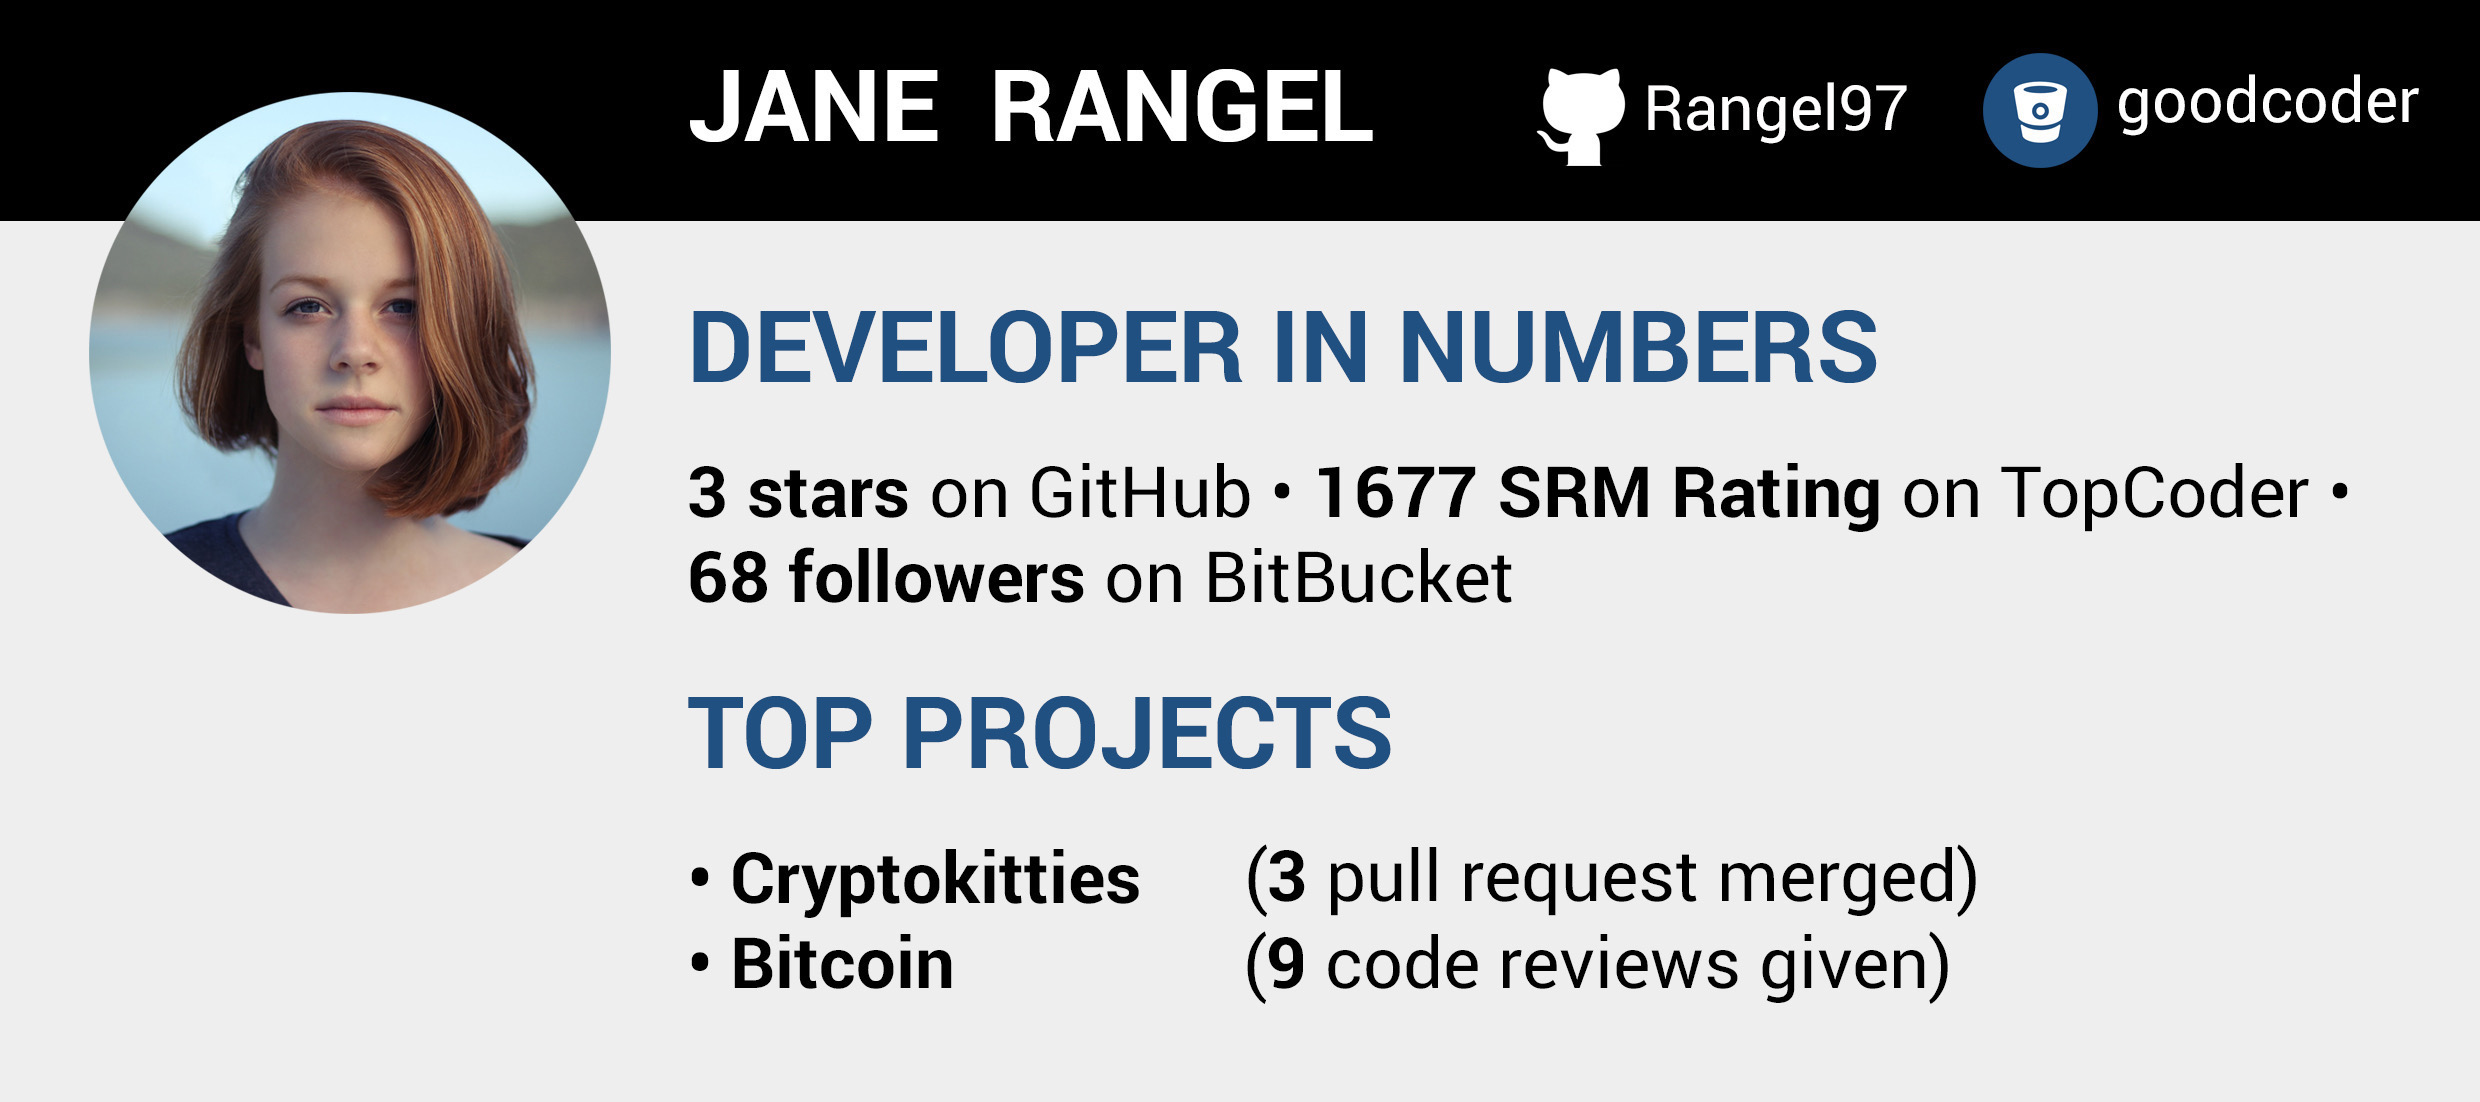
\includegraphics[width=\columnwidth]{devid/resources/devid_smaller.jpeg}
	\caption{An impression of a DevID portfolio.}
	\label{fig:devid}
\end{figure}

To show the practicality of DevID, we build a competition-based platform for crowdsourcing the development of decentralized applications, named \emph{dAppCoder}.
Crowdsourcing is a relatively new model for software development, where an open call is made for the documentation, design, coding, and testing of software~\cite{latoza2016crowdsourcing}.
We believe that a single, public, and open market is preferable compared to a centralized solution with fragmentation and lock-in effects.

The main contributions of this work are tri-fold:
\begin{itemize}
	\item \emph{DevID}: a unified portfolio specifically for dApp developers, powered by a pairwise distributed ledger (Section~\ref{sec:devid_architecture}).
	\item \emph{dAppCoder}: our application to crowdsource the development of decentralized applications (Section~\ref{sec:dappcoder}).
	\item A deployment trial of DevID and dAppCoder, which demonstrates the practicality of our work (Section~\ref{sec:experiments}).
\end{itemize}

\section{Problem Description}
\label{sec:problem_description}
The main challenge is to create a digital portfolio that gives an accurate impression of the capabilities and expertise of a developer.
We now elaborate on two requirements for this portfolio and clarify the problems we have to address.

First, we require that developers are able to import existing data from other platforms into their portfolio.
This streamlines the bootstrapping process of a portfolio with relevant records.
The problem, however, is to ensure that data being imported actually belongs to the user importing it.
This is an essential requirement to ensure trustworthy portfolios.

Second, we require our developer portfolio to be independent of any trusted intermediary.
Blockchain technology is increasingly being used as middleware for building powerful decentralized applications without centralized authority.
For example, platforms like Ethereum and EOS enable developers to write and deploy smart contracts, self-executing code that enforces agreements between two or more parties~\cite{szabo1997formalizing}.
However, most blockchain fabrics are not suitable for large-scale storage of portfolio records, or for data storage in general.

Given these two requirements, the research question of this work is as follows:
\textit{How can we provide software engineers with a unified developer portfolio, efficient at storing tamper-proof and accurate data records they control themselves?}
\begin{figure}[t!]
	\centering
	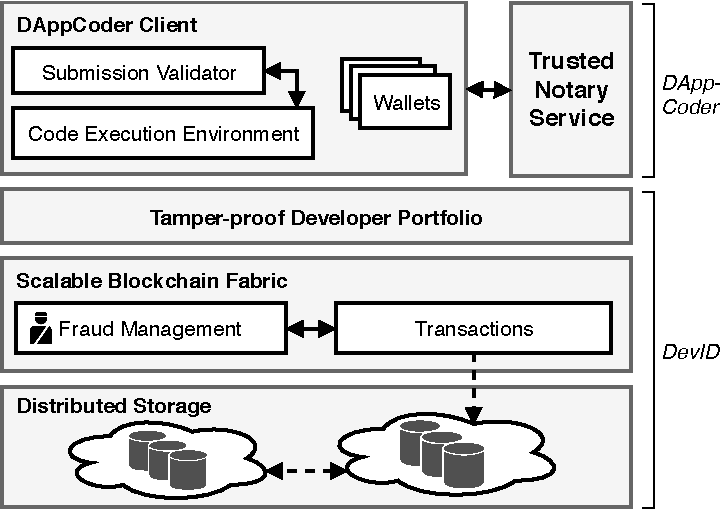
\includegraphics[width=.8\linewidth]{devid/resources/architecture.pdf}
	\caption{The architecture of DevID and dAppCoder.}
	\label{fig:system_architecture}
\end{figure}

\section{DevID: Blockchain-based Portfolios for Software Developers}
\label{sec:devid_architecture}
We now present our unified portfolio, named \emph{DevID}.
The architecture is given in Figure \ref{fig:system_architecture}.
This figure also includes the architecture of dAppCoder, our platform to crowdsource the development of decentralized applications.
dAppCoder itself is discussed in Section~\ref{sec:dappcoder}.

\subsection{Supporting Generic Storage}
We show how DevID portfolios support generic storage of records and elaborate on different record types.

\textbf{Statistics:}
The first record type we consider is statistics, quantifiable and verifiable numbers that represent a specific developer metric.
For example, these records could represent developer statistics like the number of years of programming experience, or the total number of code reviews given.
A visualization of these records is shown in Figure~\ref{fig:devid} under the section \enquote{Developer in Numbers}.

\textbf{Projects:}
Developers can add projects that they worked on to their DevID portfolio.
In Figure~\ref{fig:devid}, this information is displayed under the section \enquote{Top Projects}.
Optionally, references to projects can be added to a DevID portfolio, like a link to a GitHub repository or to the hash of a specific commit.

\textbf{Skills:}
Developers can add skills to their DevID portfolio.
We consider the ability to highlight proficiency in specific programming languages and familiarity with blockchain platforms an essential feature of a developer portfolio.
It aids programmers in finding projects that match their expertise, and it enables clients to find developers that fit their projects best.
For instance, applications that have access to DevID portfolios can filter available developers on one or multiple skills.
%Figure~\ref{fig:devid} shows two skills under the section \enquote{Programming Skills}.

\textbf{Endorsements:}
The final record type we define is endorsements.
Developers can endorse other developers (e.g., by writing a letter of recommendation) or endorse specific skills of others.
Skills and endorsements can also be imported from other platforms like LinkedIn.
How we achieve this, is discussed in the next section.

\subsection{Unifying Developer Data}
\label{subsec:unifying_data}
We now discuss how to import developer data from multiple platforms and how to verify it for correctness.

\textbf{Importing developer data:}
DevID allows developers to import relevant information from different platforms into their portfolio.
For example, they can import data from LinkedIn (e.g., skills or past projects) or from GitHub (e.g., the number of followers and code contributions).
Importing can be done by querying their public interfaces (APIs) and request the relevant data.
To store the data in the portfolio, one can either add a reference to the (external) data or copy the data assets into the portfolio.
To reduce dependency on third-party services, we choose to copy the data and store it within a portfolio record.

\textbf{Verifying developer data:}
As discussed in Section~\ref{sec:problem_description}, it is essential to ensure that imported data actually belongs to the developer importing it.
We propose two solutions to achieve trustworthy importation of data: \textit{challenges} and \textit{TLS auditing}.

The first solution is to pose a challenge where the developer importing the data, proves that they have control over this data.
For example, when importing data from GitHub, we can require a public identifier (e.g., a public key) of the developer to be part of the \enquote{bio} profile field.
This information can then be verified for correctness by other users who query the public GitHub API.
We call users who verify data \emph{witnesses}.
While this is a basic mechanism to ensure the accuracy of imported data, it heavily depends on the availability of a public API.

The second solution is TLS auditing~\cite{tlsnotary2014whitepaper}.
The key idea is to proxy a TLS connection through a random witness, which then verifies and signs the data after the TLS connection terminates.
When the TLS session finishes, the client gives the witness the private key used to decrypt HTTPS responses from the web service.
Note that this way the witness is not able to decrypt the request made to the web service, which likely includes credentials or access tokens.
The role of a witness can either be fulfilled by other entities in the network, or by a trusted notary service.
Depending on the significance of data being imported, multiple witnesses can be used for this.
Compared to challenges, TLS auditing works when access to a public API is absent but is more advanced.
Our lab has implemented an advanced TLS auditing mechanism, which is currently under a security audit.

\subsection{Verified Identities}
\label{subsec:strong_identities}
To further improve trustworthiness of DevID portfolios, developers can optionally verify their digital identity.
A verified identity is uniquely linked to a real-world entity.
Software built on DevID can give preferential treatment to developers that have verified their identity.
For example, an application can ignore endorsements that are given by unverified developers.

Identity verification can be done with an attestation given by a trusted third party like the government or a notary.
Enforcing strong, long-lived identities in DevID is comparable with account validation that many centralized platforms use (e.g., the verification of a phone number).
The requirement for verified identities addresses the Sybil Attack, where an adversary assumes multiple fake identities to influence or subvert the network~\cite{douceur2002sybil}.

\begin{figure*}[t!]
	\centering
	\begin{subfigure}[t]{.3\textwidth}
		\centering
		\captionsetup{width=.9\linewidth}
		\raisebox{4mm}{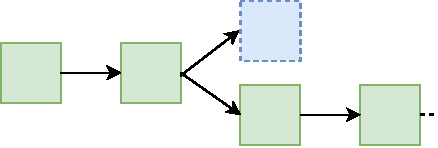
\includegraphics[width=\linewidth]{devid/resources/blockchain_single}}
		\caption{Linear ledger (Ethereum).}
		\label{fig:blockchain_single}
	\end{subfigure}\hfill%
	\begin{subfigure}[t]{.3\textwidth}
		\centering
		\captionsetup{width=.9\linewidth}
		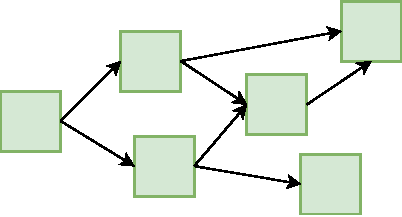
\includegraphics[width=\linewidth]{devid/resources/blockchain_dag}
		\caption{DAG ledger (IOTA).}
		\label{fig:blockchain_dag}
	\end{subfigure}\hfill%
	\begin{subfigure}[t]{.3\textwidth}
		\centering
		\captionsetup{width=.9\linewidth}
		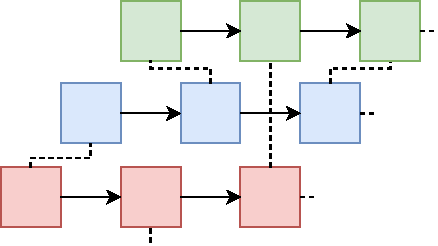
\includegraphics[width=\linewidth]{devid/resources/blockchain_pairwise}
		\caption{Pairwise ledger (Nano).}
		\label{fig:blockchain_pairwise}
	\end{subfigure}%
	\caption{Three different structures of distributed blockchain ledgers. Each arrow points to the subsequent block in the chain.}
	\label{fig:blockchain_structures}
\end{figure*}

\subsection{Efficient Blockchain Storage}
\label{subsec:scalable_blockchain}
DevID requires a blockchain fabric that can store tamper-proof and accurate data records.
We now explore three common blockchain structures, displayed in Figure~\ref{fig:blockchain_structures}.

\textbf{Linear ledger:} Figure~\ref{fig:blockchain_single} shows the linear blockchain ledger used by Ethereum.
The fundamental property of this ledger is that at least a majority of users agree on the exact sequence of transactions.
A global consensus mechanism like Proof-of-Work or Proof-of-Stake prevents the double-spend attack where a malicious user intentionally creates a fork of their chain~\cite{vukolic2015quest}.
While providing a high level of consistency, the transaction throughput of these ledgers is often not high enough to facilitate record creation and modification by millions of users.
This motivates us to consider different blockchain structures for portfolio storage.

\textbf{DAG ledger:} Another blockchain structure is the Directed Acyclic Graph (DAG) ledger, where each block can be referenced by multiple other blocks.
This ledger structure, shown in Figure~\ref{fig:blockchain_dag}, is adopted by blockchain platforms like IOTA and Dagcoin~\cite{popov2018tangle}~\cite{lerner2015dagcoin}.
IOTA is optimized for micro-payments within Internet-of-Things, and Dagcoin advertises itself as data storage for arbitrary data (e.g., documents or ownership records).
Since these ledgers allow for different consensus mechanisms, transaction throughput is often superior compared to that of linear ledgers.
However, they usually do not have the same consistency guarantees.
While these ledger structures are more suitable for data storage, we consider current implementations unfit for developer portfolios.
The reason is that they either rely on a centralized coordinator (IOTA) or a fixed group of witness nodes (Dagcoin).
Instead, our goal is to devise a portfolio infrastructure without any authority with leveraged permission.

\textbf{Pairwise Ledger:} A third blockchain structure we consider is the pairwise distributed ledger.
The key property of this ledger, given in Figure~\ref{fig:blockchain_pairwise}, is that each user maintains and grows their individual chain with transactions.
Each block holds exactly one transaction and optionally contains a (hash) pointer to a transaction in the individual chain of another user.
Blockchain fabrics like R3 Corda, Nano, and TrustChain, use pairwise ledgers as their underlying data structure~\cite{otte2017trustchain}~\cite{lemahieu2017raiblocks}~\cite{brown2017introducing}.
These platforms address the double-spending attack either by a trusted notary (Corda), a weighted voting system (Nano) or by guaranteed eventual consistency (TrustChain).
In general, they provide superior scalability compared to linear ledgers as used by Bitcoin and Ethereum but lack global consensus.

We strongly believe that the pairwise distributed ledger is a suitable data structure to store portfolio records as transactions.
Compared to linear and DAG ledgers, all data of a portfolio owner is local to their own individual ledger and maintained by themselves.
Pairwise distributed ledgers enable selective queries of data stored on the chains of other members, without the need for full data replication across the network.
In DevID, each individual ledger stores all data associated with a single portfolio, in a tamper-proof manner, and without global agreement.

\begin{figure*}[t!]
	\centering
	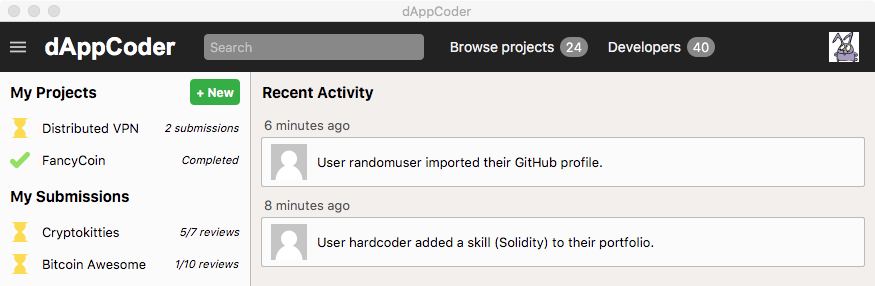
\includegraphics[width=0.99\textwidth]{devid/resources/gui_smaller.png}
	\caption{The user interface of DAppCoder, our application to crowdsource the development of decentralized applications.}
	\label{fig:dappcoder}
\end{figure*}

\subsection{Storing Large Data Assets}
While pairwise distributed ledgers are suitable for storing small portfolio records, they are not suitable for storing arbitrary large data assets.
Such data assets can include source code, documentation, and reviews.
To overcome this, we introduce an off-chain distributed storage solution that offers data immutability and scalability.
Figure~\ref{fig:system_architecture} shows the distributed storage, which comprises the lowest layer in our architecture.

Suitable distributed storage solutions for our work are a Distributed Hash Table (DHT) like Kademlia, a BitTorrent swarm or the InterPlanetary File System (IPFS)~\cite{maymounkov2002kademlia}~\cite{cohen2008bittorrent}~\cite{benet2014ipfs}.
These solutions enable users to store large data assets, without involvement of a trusted third party.
Large data is inserted in the distributed storage back-end, and a reference to the data (i.e., a content hash) is included in the on-chain transaction.

\section{dAppCoder: Crowdsourcing Development of Decentralized Applications}
\label{sec:dappcoder}
By extending the DevID portfolio architecture and record types, we create a competition-based crowdsourcing platform for the development of decentralized applications.
Running completely without servers, our platform named dAppCoder matches clients and dApp developers.
The architecture of dAppCoder is presented in the upper layer of Figure~\ref{fig:system_architecture} and the user interface is shown in Figure~\ref{fig:dappcoder}.
We now elaborate on the main functionalities of dAppCoder.

\subsection{Creating Projects}
Clients that want their idea realized (e.g., the implementation of a specific smart contract) can create a new project in dAppCoder.
Creating a new project requires the client to specify a project title, requirements, a submission deadline, the number of testers needed for each submission, and a list of skills needed to work on the project.
When creating a new project, a single portfolio record with all project information is constructed, appended to the individual ledger, and disseminated in the network.
Since the project requirements might be of arbitrary length, we store it in the distributed storage back-end and embed a pointer to it in the portfolio record.
For each new project, the client generates a \textit{project keypair}, which consists of a public and private key.
These keys are used when releasing the submissions for a project, which is discussed in Section~\ref{subsec:create_submissions}.

To incentivize developers to work on a particular project, each project has a fixed monetary reward which is disbursed by the client to the developer with the best submission.
Prior to posting a new project, the client determines the height of the reward and transfers it to a \textit{Trusted Notary Service} (shown in Figure~\ref{fig:system_architecture}).
This compensation, put into escrow, directly addresses an attack where clients flood the system with invalid or irrelevant projects.
The trusted notary can either be a centralized authority or an (Ethereum) smart contract that interacts with the dAppCoder application through oracles.

Each project goes through two phases during its lifetime: a \emph{submission} and a \emph{testing} phase.
During the submission phase, developers can create submissions for a project until the submission deadline (which is determined by the client).
The duration of the testing phase depends on the time it takes for the project to accumulate the required number of testers.

\subsection{Creating Submissions}
\label{subsec:create_submissions}
Developers looking for work can browse through the list of open projects, or filter them based on the skills they have added to their DevID portfolio.
When a developer has found an interesting project, they work towards a submission.
A submission must consist of source code and documentation, which are inserted in the distributed storage back-end.
For each submission, a new portfolio record is created with a pointer to the project and submission files.
Incoming submissions after the submission deadline has passed, will not be considered for testing.

To prevent a free-riding attack where a developer copies the solution of another participant, the content of each submission is encrypted with the (public) project key~\cite{zhang2015keep}.
To ensure that testers can decrypt submissions, the client sends the private project key to them after the submission deadline has passed.

\subsection{Testing Submissions}
\label{subsec:review_submissions}
After the submission deadline passed, all submissions should be tested by other developers.
For simplicity, we assume that the client selects appropriate testers for submissions, based on their expertise (indicated by their DevID portfolio) and the total number of submissions tested in the past.
To incentivize developers to test submissions, testing activities will be prominently displayed on their DevID portfolio.
The testing phase consists of two phases, where tests are written and verified.
To avoid collusion between developers, we require that individuals who have created a submission, written tests, and verified these tests, are not affiliated.

\textbf{Writing tests:}
First, testers write tests to verify the correctness of a submission.
These tests can be used to expose critical vulnerabilities or programming errors in business-critical code.
If a tester found such an error, they can mark the submission for exclusion and should provide a test that highlights it.

Besides writing tests, each tester grades the submission based on compliance to the specifications.
The given score can range from "very low" (-2), "low" (-1), "neutral" (0), "sufficient" (1) or "high" (2).

\textbf{Verifying tests:}
Second, developers inspect the tests, written by testers in the previous phase.
In particular, thoroughness and completeness of the tests written by a specific tester will be graded by giving a similar score as in the previous phase.

\subsection{Paying Out Developers}
\label{subsec:dappcoder_payout}
When the testing phase of a project ends, the best submission is determined by having the highest average score rating.
The developer with the best submission is compensated for the effort.
Since all reviews are public, the trusted notary service is able to transfer the reward to the eligible developer.
This reward is transferred to cryptocurrency wallets, which can be added to dAppCoder.

\section{Implementation and Deployment Trial}
\label{sec:experiments}
Next, we elaborate on the implementation of both the DevID portfolio and the dAppCoder application.
We also discuss our deployment trial and present the results.

\subsection{Our Implementation}
We have implemented both DevID and dAppCoder in the Python programming language.
Our implementation consists of all components shown in Figure~\ref{fig:system_architecture}, except for the trusted notary service.
The graphical user interface of dAppCoder is implemented with the Qt5 library and communicates with the back-end over a RESTful API.
The open source implementations of both DevID and dAppCoder are available online.\footnote{https://github.com/tribler/dappcoder}

We build DevID, and by extension dAppCoder, on the TrustChain ledger introduced by Otte et al~\cite{otte2017trustchain}.
We identified two advantages of TrustChain over other pairwise distributed ledgers like R3 Corda and Nano.
First, TrustChain focuses on fraud \emph{detection} instead of \emph{prevention} and as a result does not require network-wide consensus.
This makes TrustChain a lightweight and simple data structure.
Second, TrustChain is already used as transaction fabric within a self-sovereign, decentralized identity system, described in the work of Stokkink et al~\cite{stokkink2018deployment}.
Availability of a self-sovereign identity system aligns with our requirement for strong, long-lived identities (see Section~\ref{subsec:strong_identities}).
We use the InterPlanetary File System (IPFS) to store large data assets like project specifications, submissions and code reviews.
Users can import statistics from their GitHub profile using the challenge mechanism described in Section~\ref{subsec:unifying_data}.

\begin{figure}[t!]
	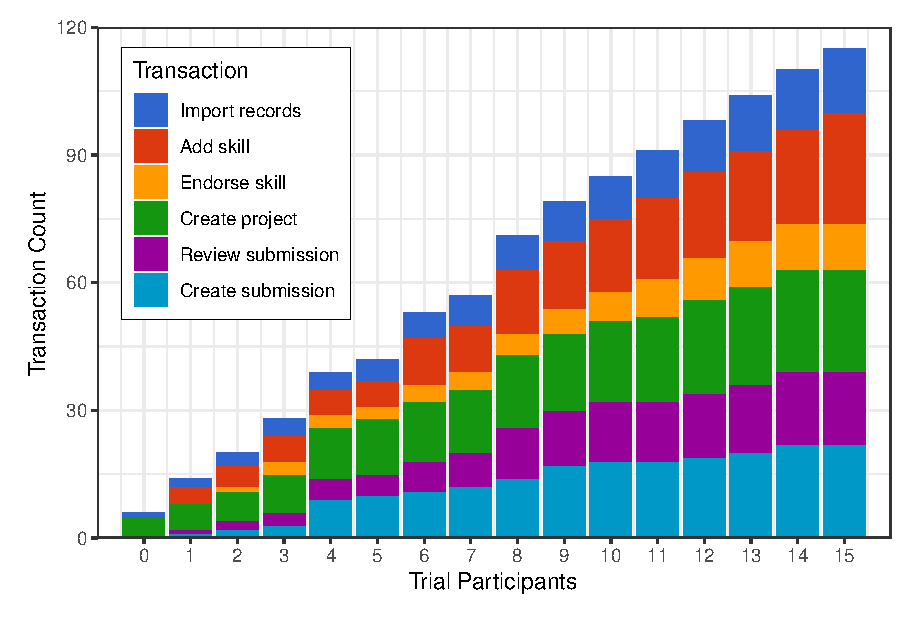
\includegraphics[width=.75\columnwidth]{devid/resources/experiment/experiment_1_unit.eps}
	\caption{Results from our deployment trial.}
	\label{fig:experiment_graph}
\end{figure}

\subsection{Deployment Trial}
To assess the feasibility of dAppCoder and to get insight into the efficiency of the TrustChain ledger, we conduct a deployment trial.
We present the trial setup and results.

\textbf{Setup:}
For our trial, we recruited 15 participants among local staff and students of our faculty.
To bootstrap the application, we initiated dAppCoder with five projects ourselves.
Two of these projects asked developers to resolve one or more bugs in a piece of Python code.
The other three projects asked the developer to implement a small application.
Since only a fraction of our users is familiar with the development of decentralized applications, we accepted submissions in other programming languages during our trial, like Java.
We collected data and observed the growth of the distributed ledger over a period of five working days.
During this time, developers were free to use the application as they see fit.

\textbf{Results:}
Figure~\ref{fig:experiment_graph} shows the growth of the TrustChain ledger when more participants join the trial.
Each entry on the horizontal axis represents the state of the ledger after a participant was introduced, and the vertical axis shows the transaction count for the six different types of transactions.
When more participants join, the distribution of transaction types on the ledger changes slightly.
We observe that the growth of projects over time decreases, and users focus more on creating submissions and reviews.
Another observation is that the number of skills added by each developer grows rapidly, but the growth of endorsements stays behind.

At the end of our deployment trial, the average transaction size in serialized form is 0.6 kB.
The total size of all transactions stored on the distributed ledger is 65.4 kB.
Each individual ledger stores on average 7.2 transactions, with an average size of 4.1 kB.
In comparison, when using a linear ledger like Bitcoin, each user is required to store the entire global ledger or parts of it.  
The time required to append new transactions to the TrustChain ledger is in the range of milliseconds and not of influence on the user experience.
The initial results of the trial look promising, and we are ready for further evaluation of dAppCoder and DevID portfolios. 

\section{Related Work}
We are the first to build a tamper-proof and unified developer portfolio, to the best of our knowledge.
Already in 1995, research has been conducted, that explores the advantages of online electronic portfolios over traditional resumes, particularly within an educational environment~\cite{riggsby1995electronic}~\cite{barrett2000electronic}.
The emergence of the open source software paradigm enabled developers to use code contributions as proof of verifiable technical expertise and to build an online reputation~\cite{riehle2015open}.
The work of Cai et al. explores how this data can be used to construct a theoretical reputation model, and what metrics would be best suited for this~\cite{cai2016reputation}.
Other work is focused on visualization tools to highlight contributions of the individual developer on platforms like GitHub or StackOverflow~\cite{jaruchotrattanasakul2016open}~\cite{saxena2017know}~\cite{chen2016supporting}.
Their research is primarily focused on the design and evaluation of models to represent the technical skills, based on data from open source projects.
The focus of this work is on combining records from different platforms and presenting them in a unified portfolio.

The evolution of crowdsourcing and the benefits are well-studied topics with an extensive literature corpus~\cite{latoza2016crowdsourcing}.
TopCoder Inc. is an example of a crowdsourcing platform where clients can outsource software contributions to developers in a competition-based environment~\cite{lakhani2010topcoder}.
In 2017, Li et al. introduced CrowdBC, a decentralized blockchain-based framework for crowdsourcing~\cite{li2017crowdbc}.
CrowdBC is a platform to crowdsource generic micro-tasks and is not suitable to crowdsource development of decentralized applications.
Lu et al. devised a privacy-preserving crowdsourcing mechanism on top of an open blockchain~\cite{lu2018zebralancer}.
Buccafurri et al. introduce TweetChain and show how to build a crowdsourcing application which stores all information on Twitter timelines~\cite{buccafurri2017tweetchain}.
TweetChain is comparable with individual ledgers in TrustChain but depends on a central authority for dissemination and storage of data (Twitter).
In comparison to most of the research performed on blockchain-based crowdsourcing, this work focuses on a specific use-case, namely crowdsourcing the development of business-critical applications.

\section{Conclusion}
We have presented DevID, a blockchain-based portfolio for developers.
DevID addresses the fragmentation and lock-in of developer data across different platforms with a mechanism to import data from third-party services.
By building upon a pairwise distributed ledger, DevID is capable of storing tamper-proof records and does not depend on any trusted party.
Portfolio records are fully managed by developers themselves.

We have proven the potential of DevID by building a crowdsourcing application for the development of decentralized applications.
Our application, dAppCoder, matches clients and reputable developers.
With a deployment trial, we have demonstrated that dAppCoder is feasible.

Future work is focused on a large-scale deployment of dAppCoder and better support for specific bug bounties.
We schedule to release in the first quarter of 2019.
Using our TLS auditing mechanism, we plan to expand DevID with additional record importation from other platforms, in particular, LinkedIn and StackOverflow.
Finally, we aim to explore the use of DevID within other domains besides crowdsourcing.